%% LyX 2.2.3 created this file.  For more info, see http://www.lyx.org/.
%% Do not edit unless you really know what you are doing.
\documentclass[oneside,italian]{book}
\usepackage[T1]{fontenc}
\usepackage[latin9]{luainputenc}
\usepackage{geometry}
\geometry{verbose,tmargin=2.5cm,bmargin=2cm,lmargin=2cm,rmargin=2cm}
\setcounter{secnumdepth}{3}
\setcounter{tocdepth}{3}

\makeatletter

%%%%%%%%%%%%%%%%%%%%%%%%%%%%%% LyX specific LaTeX commands.
%% Because html converters don't know tabularnewline
\providecommand{\tabularnewline}{\\}

%%%%%%%%%%%%%%%%%%%%%%%%%%%%%% User specified LaTeX commands.
\usepackage{listings,xcolor,courier,bookmark}
\usepackage{listingsutf8}
\definecolor{darkblue}{named}{blue}
\definecolor{darkred}{named}{red}
\definecolor{grau}{named}{gray}
\let\Righttorque\relax
\lstset{
captionpos=b,
commentstyle=\color[rgb]{0.133,0.545,0.133},
keywordstyle=\color{darkblue},
stringstyle=\color{darkred},
extendedchars=true,
basicstyle=\small\ttfamily,
showstringspaces=false,
tabsize=2,
numbers=left,
numberstyle=\tiny,
breakautoindent  = true,
breakindent      = 2em,
breaklines       = true,
postbreak        = ,
prebreak         = \raisebox{-.8ex}[0ex][0ex]{\Righttorque},
showspaces=false, 
showtabs=false, 
showstringspaces=false,
language=VHDL,
frame=single,
morecomment=[s]{--}
}


\renewcommand*{\lstlistingname}{Codice Componente}


\usepackage{fancyhdr}
\pagestyle{fancy}

\fancyhead{} 
\fancyfoot{} 

\fancyhead[RO,LE]{\bfseries \leftmark}
\fancyfoot[LE,RO]{\thepage}
\fancyfoot[LO,CE]{Tesina in ASE: Architetture dei Sistemi di Elaborazione}
\renewcommand{\headrulewidth}{0.4pt}
\renewcommand{\footrulewidth}{0.4pt}

\date{}
\cfoot{}

\makeatother

\usepackage{babel}
\begin{document}

\section{Soluzione}

\begin{tabular}{|c|c|c|c|}
\hline 
Numero di bit operandi & Numero di slice & Numero di four LUT & Tempo di calcolo\tabularnewline
\hline 
\hline 
4 & 6 & 8 & 7,225 ps\tabularnewline
\hline 
8 & 12 & 16 & 7,735 ps\tabularnewline
\hline 
16 & 24 & 32 & 9,358 ps\tabularnewline
\hline 
32 & 48 & 64 & 9,985 ps\tabularnewline
\hline 
\end{tabular}

Secondo le formule dell' area e del ritardo, l' area � pari a 5$n$
volte(dove $n$ indica il numero di full-adder) , ed 2$/delta$ $n$
per il ritardo, la realizzazione per FPGA invece ci da dimensioni
e ritardi diversi, difatti l' area raddoppia se raddoppiano il numero
di bit per la somma, molto probabilmente perch� essendoci un full\_adder
in ogni slice utilizzer� di ognuna di esse un full\_adder, invece
il tempo di calcolo all' aumentare del numero di bit cresce ma meno
che linearmente, determinante dal fatto che il sintetizzatore riuscir�
a disporre le slice molto vicine tra di loro e il tempo di propagazione
dei riporti diverr� molto piccolo, si nota per� che da 8 a 16 bit
il tempo di calcolo incrementa di una quantit� relativamente pi� grande
rispetto tra 4 e 8 o 16 e 32, forse perch� le connessione non avvengono
tra CLB vicine tra loro, per determinare il tempo si � scelto come
input sempre il massimo valore accettabile in ingresso.

Non � stato possibile testare il componente con numero di bit di operandi
a 64 bit, poich� quando si cerca di mappare sulla scheda i vari pin
di ingresso e di uscita dell ' addizionatore, questa operazione non
riesce, una soluzione sarebbe quella di evitare che I/O venga mappato,
per� ISE ci avverte che i tempi di propagazione potrebbero essere
non veritieri, allora si potrebbe utilizzare un altro componente per
far passare gli input non contemporaneamente all' addizionatore, ma
l' area del dispositivo verrebbe influenzata da tutte le connessioni
che occorrono per questo dispositivo e ci potrebbero essere delle
ottimizzazioni che minimizzano l' area.

\subsection{Schematici}

\begin{figure}[H]
	\centering
	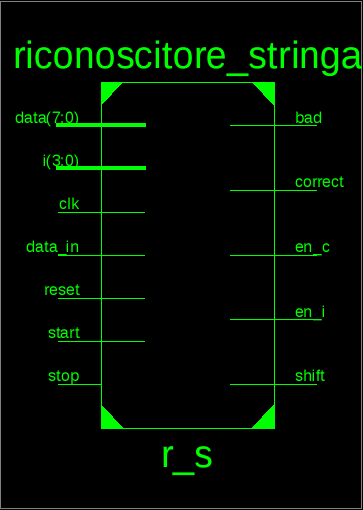
\includegraphics[scale=0.7]{esercizio07/images/riconoscitore_stringa.png}
	\caption{Ripple_carry_adder}
\end{figure}

\subsection{Codice}

\href{run:progetti/RippleCarryAdder/RippleCarryAdder.xise}{RippleCarryAdder}
\end{document}
